\section{\texorpdfstring{RSA}{RSA}}
\vspace{5mm}
\large

Setup:
\begin{itemize}
	\item $p,q$ big random primes.
	\item $n:= pq$
	\item $\varphi(n) = (q - 1)(p - 1)$
	\item $(e, \varphi(n)) = 1$ is an encryption exponent
	\item select decryption exponent $d$ s.t $ed = 1 \mod(\varphi(n))$
	\item $(e, n)$ is an enc key, $(d, n)$ is an dec key
\end{itemize}

Then we encrypt by calculating $E(X) = x^e \mod n$ and decrypt $E(y) = y^d \mod n$.
Assuming $(x, n) = 1$, last equality by the Euler theorem
\[ (x^e)^d \equiv x^{ed} \equiv x^{1 + k\varphi(n)} \equiv x \cdot x^{k \varphi(n)} \equiv x \cdot (x^{\varphi(n)})^k \equiv x \]

Therefore, encryption using RSA is invertible.
Relies on the hardness of factorisation.

RSA is slow, but polynomial. Which leads to hybrid ciphers.
However, we can made some adjustments to improve computations:
\begin{itemize}
	\item choose small public exponent (3, 17, $65537 = 2^{16} + 1$)
	\item use CRT for private calculations (compute mod p, mod q and combine using CRT)
\end{itemize}

\begin{properties} RSA
\begin{itemize}
	\item Commutative: $D_2(D_1(E_2(E_1(x)))) = x$.
	\item Homomorphic: $E(x_1 x_2) = (x_1 x_2)^e = x_1^e x_2^e = E(x_1) E(x_2)$.
\end{itemize}
\end{properties}

\begin{example}
	RSA usage for \textbf{Blind signature}:

	Firstly, Alice signs some text. Bob want to sign message secretely from Alice. Steps:
	\begin{enumerate}
		\item Bob generates $b \in_R \Z_n^{\ast}$, sends $x b^d$ to Alice
		\item Alice sends back $(x b^d)^e = x^e b$
		\item Bob calculates $x^e b b^{-1} = x^e$ and gets the signature done by Alice.
	\end{enumerate}
\end{example}

\begin{definition}
	Semantic security - any properties of the plain text cannot be efficienlty computed from cipher text.
\end{definition}

\paragraph{Attacks on RSA}
\begin{enumerate}
	\item If $x < \sqrt[e]{n} \Rightarrow$ decrypt is e-th root in $\Z_n$, not that hard.
	\item If anybody knows $\varphi(n) \Rightarrow$ he can factorise $n$.
	\item If anybody knows $e,d \Rightarrow$ he can factorise $n$.
	\item Wiener. If $d < \sqrt[4]{n} \Rightarrow$ d could be obtained from $e$ probabilistically.
	\item Meet in the meedle: we know $c = m^e$, $e$ is also public. Try random small $u, v$ to get a collision.
		Then
		\[ u^e \equiv c v^{-e} \iff u^e v^e = m^e \iff (uv)^e \equiv m^e \Rightarrow ev = m \]
	\item similar massages: $m, (m + \delta)$.
		\[ c = m^e \land c^{\prime} = (m + \delta)^e \iff P(m) = m^e - c \land P^{\prime}(m) = (m + \delta)^e - c^{\prime} \]
			Therefore, $m$ is the root of 2 polynomials.
			If $e$ is small $\Rightarrow P, P^{\prime}$ have small degree and $m$ is a root of $gcd(P, P^{\prime})$.
			Which is a linear polynomial with high probability.

			Alternatively, the attacker can guess $\delta$.
	\item $p$ and $q$ are close to each other $\Rightarrow$ easier factorisation of $n$.
	\item single message encrypted with the same e but different mod.
		Ex: $e = 3, n_1, n_2, n_3$ are 3 different residuals
		\begin{gather*}
			x^3 = y_1 \mod n_1\\
			x^3 = y_2 \mod n_2\\
			x^3 = y_3 \mod n_3
		\end{gather*}
		So, \[x < \min(n_1, n_2, n_3) \Rightarrow x^3 < n_1n_2n_3\] and $x^3$ can be calculated using CRT. Then, cubic root.

		Solutions: high $e$ or randomize messages.
	\item Not 100\% Semantic secure, as RSA leaks Jacobi Symbol
		\[ \left(\frac{x}{p}\right) \left(\frac{x}{q}\right) \]
		Which is approximately 1 bit of information.

	However, computing parity of $x$ from $E(x)$ is equivalent to full decryption.
\end{enumerate}

To avoid many pitfals of RSA design, we can use Padding scheme.
\begin{itemize}
	\item PKCS v1.5: mix message and random bits:

		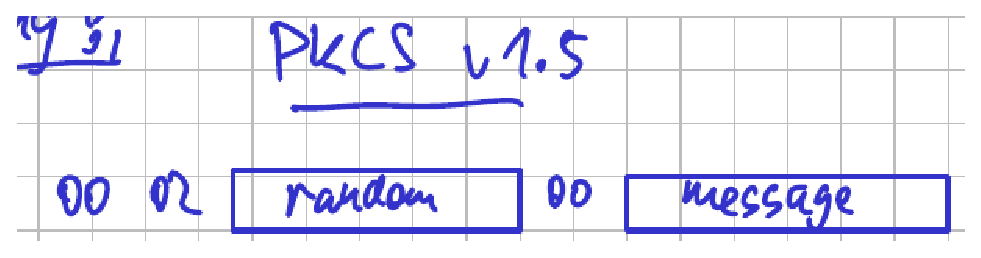
\includegraphics[scale=0.4]{pkcs_0.eps}

		There exists a oracle padding attack, Bleichenbacher.
	\item PKCS v2: add 2 hash functions and XORs (2 Feistel networks)

		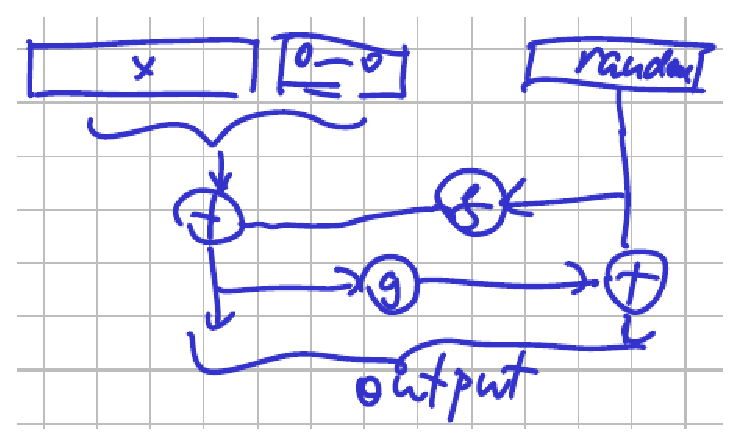
\includegraphics[scale=0.4]{pkcs_1.eps}

		Proved to be secure against oracle padding attack.
\end{itemize}

\subsection{Diffie-Hellman key exchange protocol}
Parameters:\\
1) $p$ is a prime\\
2) $\langle g \rangle = \Z_p^{\ast}$ generator

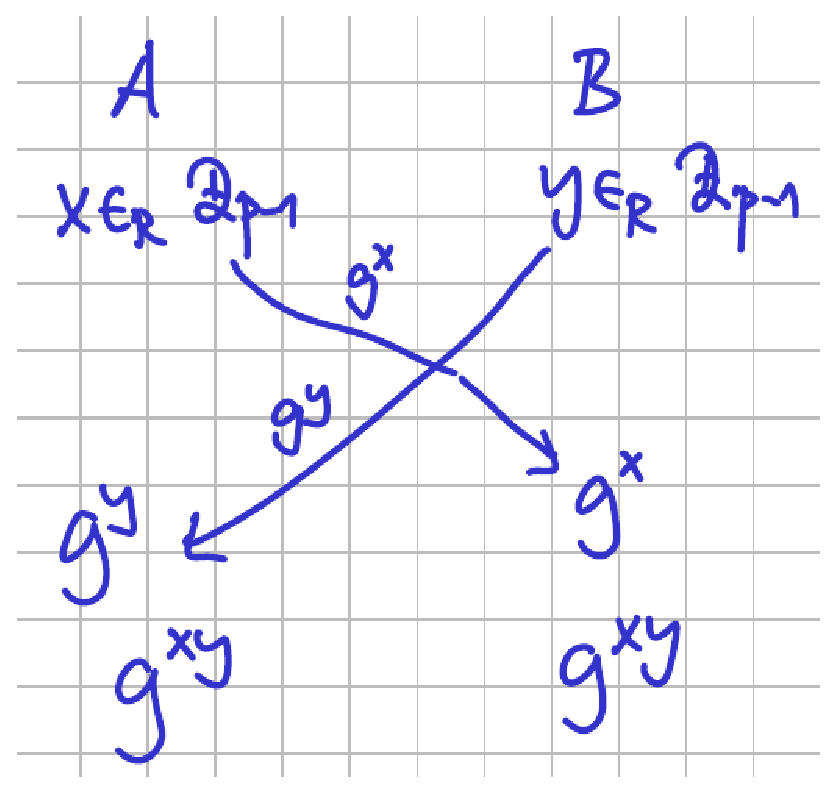
\includegraphics[scale=0.4]{dh.eps}

Problems:
\begin{itemize}
	\item Man-in-the-middle could alter messages. Solution: sign the result
	\item Attack on parameters: replace $g$ by $g^k$ which generates only a subgroup of $H \leq \Z_p^{\ast}$
		Solution: check the parameters.
	\item Powering attack: Mallory replaces $g^x$ sent by Bob by $g^{kx}$, similarly for Alice.
		Computed signature on both sides still matches, however we are in the smaller subgroup again.
		Whick makes finding the generator much easier.

		Solution: sign the whole communication.
	\item D-H leaks whether $g^{xy}$ is a quadratic residue, $<$ 1 bit leak
	\item Common trick to fix subgroup attacks: choose safe prime $p = 2q - 1$.
		From Lagrange theorem, there are only 2 non trivial subgroups, larger of them is subgroup of quadratic residues. Easy to check.
\end{itemize}

\paragraph{El Gamal cipher based on D-H}
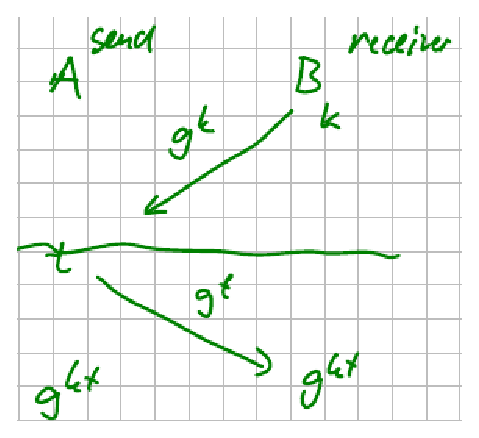
\includegraphics[scale=0.4]{dh_1.eps}

\begin{itemize}
	\item Params: prime $p$, $\langle g \rangle = \Z_p^{\ast}$ generator
	\item Keys: $k \in_R \{ 0, ..., p-2 \}$ secret.
		$h = g^k \mod p$ public
	\item Enc: $t \in_R \{ 0, ..., p-2 \}$
		\[ s = h^t = g^{kt} \mod p, y = xs \]
		Send $(g^t, y)$.
	\item Dec: Calculate $(g^t)^k$
		\[ x = y \cdot s^{-1} \mod p \]
\end{itemize}

\begin{note}
	We can also use different Algebraic structures with even harder descrete log, e.g. Elliptic curves.
\end{note}
